\documentclass[aspectratio=169,10pt]{beamer}
\usetheme{Madrid}
\usepackage[T1]{fontenc}
\usepackage{lmodern}
\usepackage{tikz}
\usepackage{adjustbox}
\usetikzlibrary{arrows.meta,positioning,fit,backgrounds,calc,shadows,shapes.geometric}

% PrismSpace Modern Technical palette
\definecolor{prismNavy}{RGB}{11,31,58}
\definecolor{prismBlue}{RGB}{0,168,198}
\definecolor{prismTeal}{RGB}{22,138,114}
\definecolor{prismMint}{RGB}{221,244,247}
\definecolor{prismGold}{RGB}{217,154,34}
\definecolor{prismDark}{RGB}{23,32,42}
\definecolor{prismLight}{RGB}{244,248,251} % ice-frost white
\definecolor{prismIndigo}{RGB}{23,54,93}
\definecolor{prismSlate}{RGB}{102,112,133}
\definecolor{cardBg}{RGB}{255,255,255}

% Harmonious pastel node fills
\definecolor{cInput}{RGB}{231,233,236}
\definecolor{cStem}{RGB}{220,214,247}
\definecolor{cStage1}{RGB}{191,232,213}
\definecolor{cStage2}{RGB}{246,213,138}
\definecolor{cStage3}{RGB}{242,184,181}
\definecolor{cStage4}{RGB}{191,227,242}
\definecolor{cHead}{RGB}{216,197,232}
\definecolor{cOutput}{RGB}{234,207,213}
\definecolor{cTask}{RGB}{231,233,236}
\definecolor{cPlanner}{RGB}{207,199,242}
\definecolor{cDispatch}{RGB}{169,220,235}
\definecolor{cReact}{RGB}{169,222,200}
\definecolor{cTool}{RGB}{244,213,141}
\definecolor{cSafety}{RGB}{240,170,167}
\definecolor{cMemory}{RGB}{214,185,230}
\definecolor{cDeliverable}{RGB}{185,222,210}

\setbeamercolor{frametitle}{bg=prismNavy,fg=white}
\setbeamercolor{background canvas}{bg=prismLight}
\setbeamertemplate{navigation symbols}{}
\setbeamertemplate{footline}{\hfill\textbf{PrismSpace} $\cdot$ CSE, CEK\hspace{1em}|\hspace{1em}\insertframenumber/\inserttotalframenumber\hspace{1.5em}\vspace{0.4em}}

\begin{document}
\begin{frame}[t]{02. System Architecture: 6-Tier Stack \& Multi-Agent Workflow}
\vspace{-0.4em}
\centering
\adjustbox{max width=0.99\linewidth, max height=0.90\textheight}{%
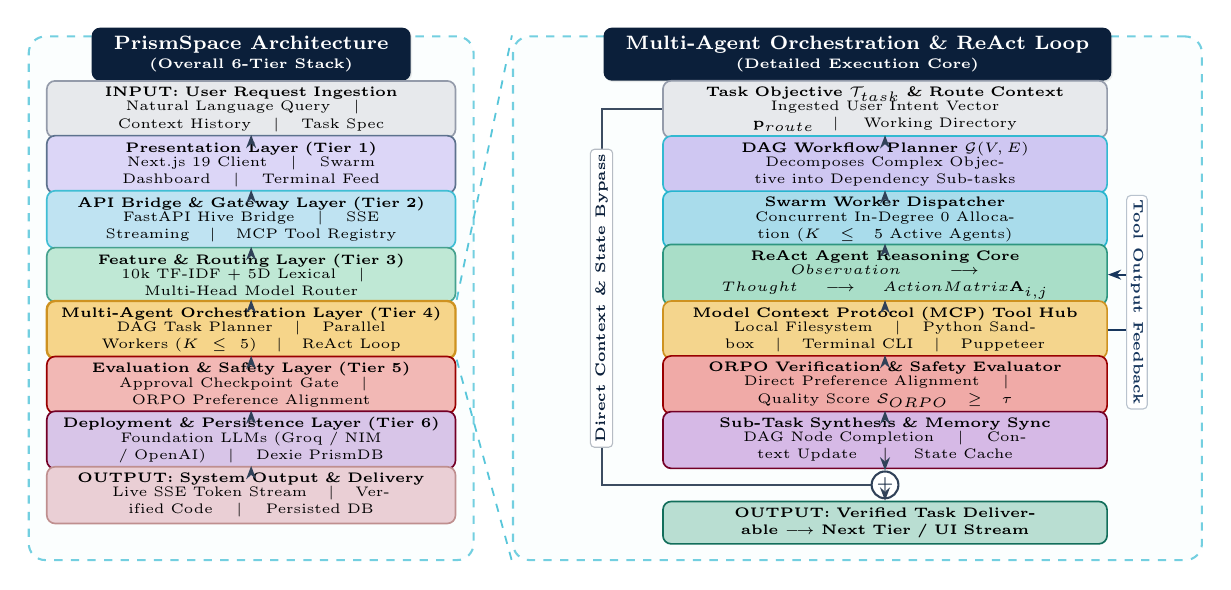
\begin{tikzpicture}[
  x=1cm, y=1cm,
  every node/.style={align=center},
  card/.style={
    draw=prismBlue!55, dashed, line width=0.75pt, fill=prismBlue!1.5,
    rounded corners=6pt
  },
  pilltitle/.style={
    fill=prismNavy, text=white, font=\scriptsize\bfseries,
    rounded corners=3pt, inner xsep=8pt, inner ysep=3.2pt,
    drop shadow={opacity=0.15, shadow xshift=0.5pt, shadow yshift=-0.5pt}
  },
  layerbox/.style={
    rectangle, rounded corners=3pt, line width=0.6pt,
    text width=5.05cm, minimum height=0.45cm, inner ysep=2.2pt, inner xsep=2pt,
    font=\fontsize{5.2}{6.2}\selectfont
  },
  detailbox/.style={
    rectangle, rounded corners=3pt, line width=0.6pt,
    text width=5.5cm, minimum height=0.45cm, inner ysep=2.2pt, inner xsep=2pt,
    font=\fontsize{5.2}{6.2}\selectfont
  },
  arrow/.style={
    -{Stealth[scale=0.75]}, line width=0.75pt, draw=prismNavy!85
  },
  conn/.style={
    draw=prismNavy!80, line width=0.75pt
  },
  zoomline/.style={
    draw=prismBlue!65, dashed, line width=0.65pt
  },
  plusnode/.style={
    circle, draw=prismNavy!85, line width=0.75pt, fill=white,
    inner sep=0pt, minimum size=0.34cm, font=\scriptsize\bfseries, text=prismNavy
  }
]

  % =========================================================================
  % LEFT CONTAINER: OVERALL 6-TIER ARCHITECTURE
  % =========================================================================
  \node[card, minimum width=5.65cm, minimum height=6.65cm] (card1) at (3.0, 3.25) {};
  \node[pilltitle] (title1) at (3.0, 6.35) {PrismSpace Architecture\\[-0.15em]{\fontsize{4.8}{5.8}\selectfont (Overall 6-Tier Stack)}};

  \node[layerbox, fill=cInput, draw=prismSlate!70] (l0) at (3.0, 5.65) {
    \textbf{INPUT: User Request Ingestion}\\[-0.15em]
    \fontsize{4.5}{5.5}\selectfont Natural Language Query $\;\vert\;$ Context History $\;\vert\;$ Task Spec
  };

  \node[layerbox, fill=cStem, draw=prismIndigo!70] (l1) at (3.0, 4.95) {
    \textbf{Presentation Layer (Tier 1)}\\[-0.15em]
    \fontsize{4.5}{5.5}\selectfont Next.js 19 Client $\;\vert\;$ Swarm Dashboard $\;\vert\;$ Terminal Feed
  };

  \node[layerbox, fill=cStage4, draw=prismBlue!75] (l2) at (3.0, 4.25) {
    \textbf{API Bridge \& Gateway Layer (Tier 2)}\\[-0.15em]
    \fontsize{4.5}{5.5}\selectfont FastAPI Hive Bridge $\;\vert\;$ SSE Streaming $\;\vert\;$ MCP Tool Registry
  };

  \node[layerbox, fill=cStage1, draw=prismTeal!80] (l3) at (3.0, 3.55) {
    \textbf{Feature \& Routing Layer (Tier 3)}\\[-0.15em]
    \fontsize{4.5}{5.5}\selectfont 10k TF-IDF + 5D Lexical $\;\vert\;$ Multi-Head Model Router
  };

  \node[layerbox, fill=cStage2, draw=prismGold!95!black, line width=0.85pt] (l4) at (3.0, 2.85) {
    \textbf{Multi-Agent Orchestration Layer (Tier 4)}\\[-0.15em]
    \fontsize{4.5}{5.5}\selectfont DAG Task Planner $\;\vert\;$ Parallel Workers ($K \le 5$) $\;\vert\;$ ReAct Loop
  };

  \node[layerbox, fill=cStage3, draw=red!60!black] (l5) at (3.0, 2.15) {
    \textbf{Evaluation \& Safety Layer (Tier 5)}\\[-0.15em]
    \fontsize{4.5}{5.5}\selectfont Approval Checkpoint Gate $\;\vert\;$ ORPO Preference Alignment
  };

  \node[layerbox, fill=cHead, draw=purple!60!black] (l6) at (3.0, 1.45) {
    \textbf{Deployment \& Persistence Layer (Tier 6)}\\[-0.15em]
    \fontsize{4.5}{5.5}\selectfont Foundation LLMs (Groq / NIM / OpenAI) $\;\vert\;$ Dexie PrismDB
  };

  \node[layerbox, fill=cOutput, draw=pink!75!black] (l7) at (3.0, 0.75) {
    \textbf{OUTPUT: System Output \& Delivery}\\[-0.15em]
    \fontsize{4.5}{5.5}\selectfont Live SSE Token Stream $\;\vert\;$ Verified Code $\;\vert\;$ Persisted DB
  };

  % Downward arrows on Left Card
  \draw[arrow] (l0) -- (l1);
  \draw[arrow] (l1) -- (l2);
  \draw[arrow] (l2) -- (l3);
  \draw[arrow] (l3) -- (l4);
  \draw[arrow] (l4) -- (l5);
  \draw[arrow] (l5) -- (l6);
  \draw[arrow] (l6) -- (l7);

  % =========================================================================
  % RIGHT CONTAINER: DETAILED VIEW (MULTI-AGENT ORCHESTRATION & REACT LOOP)
  % =========================================================================
  \node[card, minimum width=8.75cm, minimum height=6.65cm] (card2) at (10.7, 3.25) {};
  \node[pilltitle] (title2) at (10.7, 6.35) {Multi-Agent Orchestration \& ReAct Loop\\[-0.15em]{\fontsize{4.8}{5.8}\selectfont (Detailed Execution Core)}};

  % Nodes on Right Card centered at x=11.05
  \node[detailbox, fill=cTask, draw=prismSlate!70] (d_in) at (11.05, 5.65) {
    \textbf{Task Objective $\mathcal{T}_{\text{task}}$ \& Route Context}\\[-0.15em]
    \fontsize{4.5}{5.5}\selectfont Ingested User Intent Vector $\mathbf{p}_{\text{route}} \;\vert\;$ Working Directory
  };

  \node[detailbox, fill=cPlanner, draw=prismBlue!80] (d_plan) at (11.05, 4.95) {
    \textbf{DAG Workflow Planner $\mathcal{G}(V, E)$}\\[-0.15em]
    \fontsize{4.5}{5.5}\selectfont Decomposes Complex Objective into Dependency Sub-tasks
  };

  \node[detailbox, fill=cDispatch, draw=prismBlue!85] (d_disp) at (11.05, 4.25) {
    \textbf{Swarm Worker Dispatcher}\\[-0.15em]
    \fontsize{4.5}{5.5}\selectfont Concurrent In-Degree 0 Allocation ($K \le 5$ Active Agents)
  };

  \node[detailbox, fill=cReact, draw=prismTeal!90] (d_react) at (11.05, 3.55) {
    \textbf{ReAct Agent Reasoning Core}\\[-0.15em]
    \fontsize{4.5}{5.5}\selectfont $\text{Observation} \;\longrightarrow\; \text{Thought} \;\longrightarrow\; \text{Action Matrix } \mathbf{A}_{i,j}$
  };

  \node[detailbox, fill=cTool, draw=prismGold!95!black] (d_mcp) at (11.05, 2.85) {
    \textbf{Model Context Protocol (MCP) Tool Hub}\\[-0.15em]
    \fontsize{4.5}{5.5}\selectfont Local Filesystem $\;\vert\;$ Python Sandbox $\;\vert\;$ Terminal CLI $\;\vert\;$ Puppeteer
  };

  \node[detailbox, fill=cSafety, draw=red!60!black] (d_eval) at (11.05, 2.15) {
    \textbf{ORPO Verification \& Safety Evaluator}\\[-0.15em]
    \fontsize{4.5}{5.5}\selectfont Direct Preference Alignment $\;\vert\;$ Quality Score $\mathcal{S}_{\text{ORPO}} \ge \tau$
  };

  \node[detailbox, fill=cMemory, draw=purple!60!black] (d_agg) at (11.05, 1.45) {
    \textbf{Sub-Task Synthesis \& Memory Sync}\\[-0.15em]
    \fontsize{4.5}{5.5}\selectfont DAG Node Completion $\;\vert\;$ Context Update $\;\vert\;$ State Cache
  };

  \node[plusnode] (plus) at (11.05, 0.88) {$+$};

  \node[detailbox, fill=cDeliverable, draw=prismTeal!80!black, minimum height=0.38cm] (d_out) at (11.05, 0.40) {
    \textbf{OUTPUT: Verified Task Deliverable $\longrightarrow$ Next Tier / UI Stream}
  };

  % Downward arrows on Right Card
  \draw[arrow] (d_in) -- (d_plan);
  \draw[arrow] (d_plan) -- (d_disp);
  \draw[arrow] (d_disp) -- (d_react);
  \draw[arrow] (d_react) -- (d_mcp);
  \draw[arrow] (d_mcp) -- (d_eval);
  \draw[arrow] (d_eval) -- (d_agg);
  \draw[arrow] (d_agg) -- (plus);
  \draw[arrow] (plus) -- (d_out);

  % =========================================================================
  % RESIDUAL / ITERATIVE FEEDBACK LOOP (LEFT & RIGHT SIDES OF RIGHT CARD)
  % =========================================================================
  % Direct Context & State Bypass (Left side of right card)
  \draw[conn] (d_in.west) -- (7.45, 5.65) -- (7.45, 0.88) -- (plus.west);
  \node[font=\fontsize{4.4}{5.4}\selectfont\bfseries, text=prismNavy, fill=white, draw=prismNavy!30, line width=0.4pt, rounded corners=1.5pt, inner sep=1.8pt] 
    at (7.45, 3.25) [rotate=90] {Direct Context \& State Bypass};

  % Iterative ReAct tool feedback loop (Right side of right card)
  \draw[arrow, draw=prismIndigo, line width=0.75pt] (d_mcp.east) -- (14.25, 2.85) -- (14.25, 3.55) -- (d_react.east);
  \node[font=\fontsize{4.2}{5.2}\selectfont\bfseries, text=prismIndigo, fill=white, draw=prismIndigo!30, line width=0.4pt, rounded corners=1.5pt, inner sep=1.5pt]
    at (14.25, 3.20) [rotate=-90] {Tool Output Feedback};

  % =========================================================================
  % ZOOM PROJECTION LINES FROM LAYER 4 (TIER 4) TO RIGHT CARD
  % =========================================================================
  \draw[zoomline] (l4.north east) -- (card2.north west);
  \draw[zoomline] (l4.south east) -- (card2.south west);

\end{tikzpicture}%
}
\end{frame}
\end{document}
